\documentclass[12pt, a4paper]{report}
\usepackage[utf8]{inputenc}
\usepackage{enumitem}
\usepackage{algpseudocodex}
\usepackage{graphicx}
\graphicspath{ {./images/} }

\usepackage{wasysym}
\usepackage[
backend=biber,
style=alphabetic,
sorting=ynt
]{biblatex}
\addbibresource{tesina.bib}

\usepackage[pdfpagelabels]{hyperref}
\hypersetup{
    plainpages=false,
    colorlinks=true,
    citecolor=blue,
    linkcolor=blue,
    urlcolor=blue,
    filecolor=magenta,
}

\title{Tesina}
\author{Iñaki Garay}
\date{Septiembre 2020}

\begin{document}

\pagenumbering{Alph}
\begin{titlepage}
\maketitle
\thispagestyle{empty}
\end{titlepage}

\pagenumbering{arabic}
\tableofcontents
\thispagestyle{empty}

\newpage

\addcontentsline{toc}{chapter}{Introducción / Esquema General}
\chapter*{Introducción / Esquema General}

\begin{itemize}[noitemsep]

\item Los compiladores tradicionales tienen una arquitectura de pipeline.

\item Dos requerimientos nuevos paralelos: minimizar tiempo de compilacion y proveer mas informacion de manera mas interactiva a las herramientas de edicion.

\item Los editores y entornos de desarrollo modernos usan LSP (Language Server Protocol). Porque?

\item Una implementacion de LSP require de componentes de compiladores (especialmente analisis).

\item La arquitectura de pipeline no se adapta bien a estos requerimientos modernos de reducir tiempos de compilacion y de proveer informacion online durante edicion.

\item Estos objetivos puede ser logrados mediante compilacion incremental.

\item La compilacion incremental puede ser lograda mediante una arquitectura basada en queries.

\item La arquitectura basada en queries es implementada tomando inspiracion de build systems.

\item Como funciona el sistema de queries de rustc?

\item Rust-analyzer es la segunda implementacion de LSP para rust.

\item Porque no funciono la primera iteracion?

\item Rust-Analyzer usa una libreria, Salsa, para cachear las queries parciales.

\item Como funciona Salsa?

\end{itemize}

\addcontentsline{toc}{chapter}{Motivaciones}
\chapter*{Motivaciones}

Los compiladores ya no son cajas negras que ingestan un conjunto de archivos fuente y producen codigo ensamblador.
De compiladores modernos se espera que:

\begin{itemize}[noitemsep]
\item Sean incrementales, es decir, si se recompila el proyecto despues de producir modificaciones en el código fuente, solo se recompila lo que fue afectado por esas modificaciones.

\item Provean funcionalidad para editores, e.g. saltar a definición, encontrar el tipo de una expresión en una ubicación dada, y mostrar errores al editar.
\end{itemize}

\addcontentsline{toc}{section}{Arquitecturas Tradicionales de Compiladores [Olle20]}
\section*{Arquitecturas Tradicionales de Compiladores [Olle20]}

\noindent
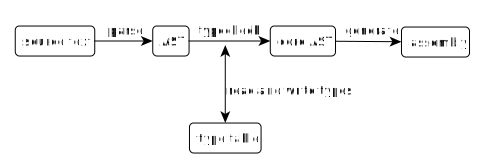
\includegraphics[width=\textwidth]{olle_trad_comp_arq}
\cite{olle_query_based}

Hay muchas variaciones, y frecuentemente mas pasos y representaciones intermedias que las ilustradas, pero la idea esencial es la misma: se empuja codigo fuente por un pipeline y corremos una sequencia fija de transformaciones hasta que finalmente emitimos codigo ensamblador o algun otro lenguaje.
En el camino frecuentemente se necesita leer y actualizar estado interno.
Por ejemplo, se puede actualizar la tabla de tipos durante la fase de verificacion de tipado, para que mas adelante se pueda verificar el tipo de las entidades a las cuales el codigo se refiere.
\cite{olle_query_based}

\addcontentsline{toc}{section}{Language Server Protocol}
\section*{Language Server Protocol}

El Language Server Protocol (LSP) es una protocolo abierto basado en JSON-RPC para el uso entre editores de codigo fuente o entornos de desarrollo integrados (IDE) y servidores que proveen funcionalidades especificas a lenguajes de programacion.
El objetivo del protocolo es permitir que se implemente y distribuya el soporte para un lenguaje de programacion independientemente de un editor o IDE determinado.
Implementar funcionalidad tal como autocompletado, ir a definicion, o mostrar documentacion relacionada a una entidad para un lenguaje de programacion determinado, requieren de esfuerzos significantes.
Tradicionalmente este trabajo se debia repetir para cada herramienta de desarrollo, dado que cada herramienta proveia un API diferente al impl
Un Servidor de Lenguaje provee inteligencia especifica a un lenguaje y se comunica con herramientas de desarrollo mediante un protocolo que permite comunicacion entre procesos.
La idea detras de LSP es estandarizar el protocolo con el cual se comunican los las herramientas de desarrollo y los servidores. De esta manera, un unico servidor de lenguaje puede ser reutilizado por multiples herramientas de desarrollo, las cuales a su vez pueden soportar multiples lenguajes, con esfuerzo minimo.
\cite{language_server_protocol}

Los entornos de desarrollo integrados (IDEs) modernos proveen a desarrolladores funcionalidad sofisticada tale como completado de codigo, refactoreo, navegacion a definicino de un simbolo, resaltamiento de sintaxis, y marcadores de errores y avisos.
Por ejemplo, en un lenguaje basado en texto, un programador podria querer renombra un metodo.
El programador podria o bien manualmente editar los archivos de codigo fuente respectivos y cambiar las ocurrencias apropiadas del nombre viejo del metodo al nuevo, o usar las capacidades para refactorear del IDE para hacer los cambios automaticamente.
Para poder soportar este tipo de refactoreo, un IDE necesita una sofisticado comprehension del lenguaje de programacion en que esta escrito el codigo.
Una herramienta de desarrollo sin ese entendimiento, por ejemplo una que hace una busqueda y reemplazo simple, podria introducir errores.
Por ejemplo, al renombrar un un metodo "read", la herramienta no deberia reemplazar identificadores como "readyState" que contienen el identificador a renombrar, ni tampoco reemplazar porciones de comentarios. Tampoco deberia suceder que renombrar una variable local afecte a variables con nombres similares en otros alcances.
\cite{language_server_protocol_wiki}

Los compiladores e interpretees convencionales son usualmente incapaces de proveer estos servicios de lenguaje, dado que estan implementados con el objetivo de o bien transformar el codigo fuente en codigo objeto o ejecutar inmediatamente el codigo.
Adicionalmente, los servicios de lenguaje deben poder manejar codigo que no esta bien formado, e.g. cuando el programador esta en el medio de editar y no ha terminado de escribir una expresion, procedimiento, u otra construccion del lenguaje.
Mas aun, pequeños cambios que ocurren durante la escritura normalmente cambian la semantica del programa.
Para poder proveer feedback instantaneo al usuario, la herramienta de edicion debe poder evaluar muy rapidamente las consequencias sintacticas y semanticas de una modificacion especifica.
Los compiladores e interpretes, por lo tanto, son pobres candidatos para la produccion de la informacion necesaria para la consumicion por una herramienta de edicion.
\cite{language_server_protocol_wiki}

Previamente al diseño e implementacion de LSP para el desarrollo de Visual Studio Code, la mayoria de los servicios de lenguaje estaban atados a un IDE o editor especifico.
En la ausencia del LSP, los servicios son tipicamente implementados utilizando un API de extension especifica a una herramienta.
Proveer el mismo servicio a otra herramienta de edicion requiere de un esfuerzo para adaptar el codigo existente para que el servicio pueda soportar las interfaces de la segunda herramienta.
\cite{language_server_protocol_wiki}

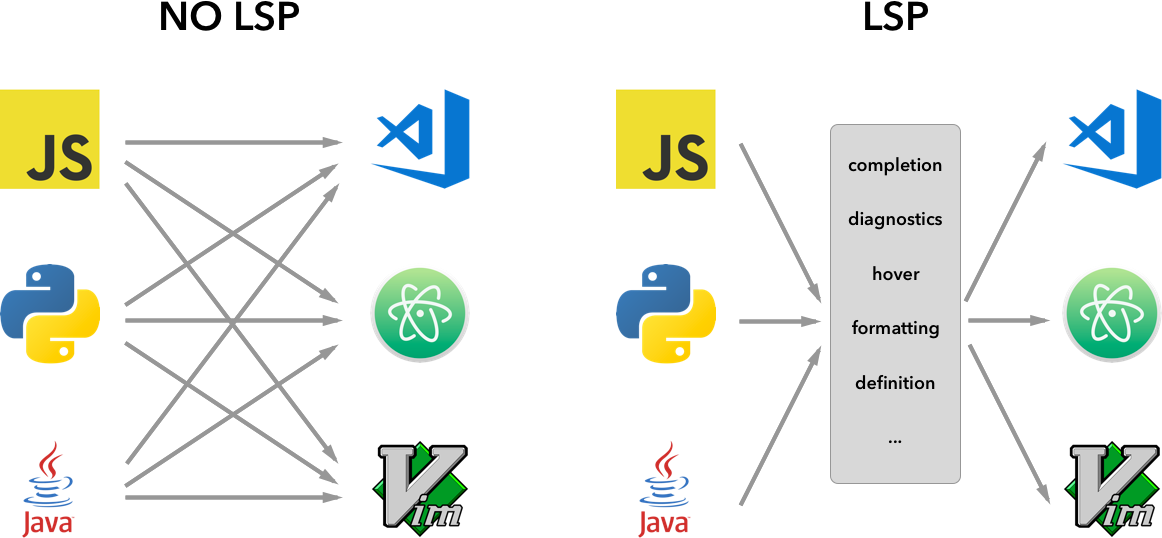
\includegraphics{lsp}

LSP permite desacoplar los servicios de lenguaje del editor de tal manera que los servicios se pueden contener en un servidor de lenguaje de proposito general.
Cual editor puede acceder a soporte sofisticado para muchos lenguajes diferentes al hacer uso de los servidores de lenguaje existentes.
Similarmente, un programador involucrado en el desarrollo de un lenguaje nuevo puede crear servicios para ese lenguaje y hacerlo inmediatamente disponible para editores existentes.
Hacer uso de servidores de lenguaje a traves del LSP por lo tanto tambien reduce la carga sobre los desarrolladores de herramientas de edicion, dado que no necesitan desarrollar sus propios servicios de lenguaje para cada lenguaje que quieren soportar.
El LSP tambien habilita la distribucion y desarrollo de servidores contribuidos por terceros, tales como usuarios finales, sin participacion ni por parte de los desarrolladores del compilador del lenguaje o por los desarrolladores de la herramienta de edicion para la cual se esta agregando soporte de lenguaje.
\cite{language_server_protocol_wiki}

LSP no se limita a lenguajes de programacion.
Puede ser utilizacion para cualquier lenguaje basado en texto, tales como lenguajes de especificacion o especificos a dominions (DSL).
\cite{language_server_protocol_wiki}

\addcontentsline{toc}{section}{Velocidad de Compilación}
\section*{Velocidad de Compilación}

Mejorar los tiempos de compilacion ha sido un foco principal despues de que Rust llego a la version 1.0.
Sin embargo, gran parte del trabajo en pos de este objetivo ha sido sentar las bases arquitectonicas dentro del compilador.

Uno de los proyectos que esta construyendo sobre esta base, y que deberia mejorar los tiempos de compilacion para flujos de trabajo tipicos es la compilacion incremental.
La compilacion incremental evita repetir trabajo cuando se compila un paquete, lo cual llevara en ultima instancia a un ciclo de edicion-compilacion-debug mas rapido.
\cite{rust_blog_incremental_compilation}

\addcontentsline{toc}{chapter}{Mecanismos}
\chapter*{Mecanismos}

\addcontentsline{toc}{section}{Compilación Incremental}
\section*{Compilación Incremental}

La compilación incremental es una forma de computación incremental aplicada a la compilación.
En contraste con compiladores comúnes que realizan "builds limpios" y ante un cambio en el código fuente recompilan todas las unidades de compilación, un compilador incremental solo recompila las unidades modificadas.
Al construir sobre el trabajo hecho previamente, el compilador incremental evita la ineficiencia de repetir trabajo ya realizado.
Se puede decir que un compilador incremental reduce la granularidad de las unidades de compilación tradicionales a la vez que mantiene la semántica del lenguaje.
\cite{wiki_incremental_compiler}

Muchas herramientas de desarrollo aprovechan compiladores incrementales para proveer a sus usuarios un entorno mucho mas interactivo.
No es inusual que un compilador incremental sea invocado por cada cambio en un archivo fuente, de tal manera que el usuario es informado inmediatamente de cualquier error de compilación causado por sus modificaciones.
Este esquema, en contraste con el modelo de compilación tradicional, acorta el ciclo de desarrollo considerablemente.
\cite{wiki_incremental_compiler}

Una desventaja de este esquema es que el compilador no puede optimizar fácilmente el código que compila, dada la localidad y el alcance reducido de los cambios.
Normalmente esto no es un problema, dado que la optimización del código generado se aplica solamente al producir un \textit{release build}, instancia en la cual se puede usar el compilador tradicional.
\cite{wiki_incremental_compiler}

\addcontentsline{toc}{section}{Arquitectura Basada en Queries [Olle20]}
\section*{Arquitectura Basada en Queries [Olle20]}

\addcontentsline{toc}{subsection}{Pasar de pipelines a queries [Olle20]}
\subsection*{Pasar de pipelines a queries [Olle20]}

Que se necesita para obtener el tipo de un identificador calificado?
En una arquitectura basada en pipelines, se buscaria el tipo en la tabla de simbolos.
Con queries, hay que pensarlo de manera distinta.
En lugar de depender de haber actualizado un fragmento de estado, se computa de cero.
En una primera iteracion, se hace siempre completamente de cero.
Primero se averigua de cual archivo viene el nombre, y luego se leen el contenido del archivo, se parsea, posiblemente se realize algo de resolucion de nombres para saber a que nombres se refiere el codigo dado lo que se importa, y por ultimo se busca la definicion cuyo nombre ha sido resuelto y se verifica su tipo, finalmente retornandolo.

\textit{We first find out what file the name comes from, then read the contents of the file, parse it, perhaps we do name resolution to find out what the names in the code refer to given what is imported, and last we look up the name-resolved definition and type check it, returning its type.}

\begin{verbatim}
fetchType :: QualifiedName -> IO Type
fetchType (QualifiedName moduleName name) = do
    fileName <- moduleFileName moduleName
    sourceCode <- readFile fileName
    parsedModule <- parseModule sourceCode
    resolvedModule <- resolveNames parsedModule
    let definition = lookup name resolvedModule
    inferDefinitionType definition
\end{verbatim}

Refactoreando este esquema en funcionas mas chicas.

\begin{verbatim}
fetchParsedModule :: ModuleName -> IO ParsedModule
fetchParsedModule moduleName = do
  fileName <- moduleFileName moduleName
  sourceCode <- readFile fileName
  parseModule moduleName

fetchResolvedModule :: ModuleName -> IO ResolvedModule
fetchResolvedModule moduleName = do
  parsedModule <- fetchParsedModule moduleName
  resolveNames parsedModule

fetchType :: QualifiedName -> IO Type
fetchType (QualifiedName moduleName name) = do
  resolvedModule <- fetchResolvedModule moduleName
  let definition = lookup name resolvedModule
  inferDefinitionType definition
\end{verbatim}

Notemos que cada una de estas funciones hace todo de cero, i.e. cada una realiza un prefijo cada vez mas largo del trabajo total que se haria en un pipeline.
Esto ha resultado ser un patron comun en compiladores basados en queries.
Una forma de mejorar la eficiencia de este esquema es agregar una capa de memoizacion alrededor de cada funcion.
De esta manera, se ejecuta trabajo

- That way, we do some expensive work the first time we
invoke a function with a specific argument, but subsequent
calls are cheap as they can return the cached result.

- This is essentially what we'll do, but we won't use a
separate cache per function, but instead have a central
cache, indexed by the query.
\cite{olle_query_based}

\addcontentsline{toc}{section}{Why Incremental Compilation in the First Place? [Woe16]}
\section*{Why Incremental Compilation in the First Place? [Woe16]}

\begin{verbatim}
- Much of a programmer's time is spent in an
  edit-compile-debug workflow:
  - you make a small change (often in a single module or
    even function),
  - you let the compiler translate the code into a binary,
    and finally
  - you run the program or a bunch of unit tests in order
    to see results of the change.

- After that it's back to step one, making the next small
change informed by the knowledge gained in the previous
iteration. This essential feedback loop is at the core of
our daily work. We want the time being stalled while waiting
for the compiler to produce an executable program to be as
short as possible.

- Incremental compilation is a way of exploiting the fact
that little changes between compiles during the regular
programming workflow: Many, if not most, of the changes done
in between two compilation sessions only have local impact
on the machine code in the output binary, while the rest of
the program, same as at the source level, will end up
exactly the same, bit for bit.

Incremental compilation aims at retaining as much of those
unchanged parts as possible while redoing only that amount
of work that actually must be redone.
\end{verbatim}
\cite{rust_blog_incremental_compilation}

\addcontentsline{toc}{section}{How Do You Make Something "Incremental"? [Woe16]}
\section*{How Do You Make Something "Incremental"? [Woe16}

\begin{verbatim}
- We have already heard that computing something
incrementally means updating only those parts of the
computation's output that need to be adapted in response to
a given change in the computation's inputs.

- One basic strategy we can employ to achieve this is to
view one big computation (like compiling a program) as a
composite of many smaller, interrelated computations that
build up on each other.

- Each of those smaller computations will yield an
intermediate result that can be cached and hopefully re-used
in a later iteration, sparing us the need to re-compute that
particular intermediate result again.
\end{verbatim}
\cite{rust_blog_incremental_compilation}

\addcontentsline{toc}{section}{An Incremental Compiler [Woe16]}
\section*{An Incremental Compiler [Woe16]}

\begin{verbatim}
- The way we chose to implement incrementality in the Rust
compiler is straightforward: An incremental compilation
session follows exactly the same steps in the same order as
a batch compilation session.

- However, when control flow reaches a point where it is
about to compute some non-trivial intermediate result, it
will try to load that result from the incremental
compilation cache on disk instead.

- If there is a valid entry in the cache, the compiler can
just skip computing that particular piece of data. Let's
take a look at a (simplified) overview of the different
compilation phases and the intermediate results they
produce:

- First the compiler will parse the source code into an
abstract syntax tree (AST). The AST then goes through the
analysis phase which produces type information and the MIR
for each function. After that, if analysis did not find any
errors, the codegen phase will transform the MIR version of
the program into its machine code version, producing one
object file per source-level module. In the last step all
the object files get linked together into the final output
binary which may be a library or an executable.

- So, this seems pretty simple so far: Instead of computing
something a second time, just load the value from the cache.
Things get tricky though when we need to find out if it's
actually valid to use a value from the cache or if we have
to re-compute it because of some changed input.
\end{verbatim}
\cite{rust_blog_incremental_compilation}

\addcontentsline{toc}{section}{Seguimiento de Dependencias [Olle20]}
\section*{Seguimiento de Dependencias [Olle20]}

\begin{verbatim}
- Rock, Shake, Salsa

- This functionality is provided by Rock, a library that
packages up some functionality for creating query-based
compilers.

- Rock is an experimental library heavily inspired by Shake
and the Build systems à la carte paper.

- It essentially implements a build system framework, like
- make.

- Build systems have a lot in common with modern compilers
since we want them to be incremental, i.e. to take advantage
of previous build results when building anew with few
changes.

- But there's also a difference: Most build systems don't
care about the types of their queries since they work at the
level of files and file systems.

- Build systems à la carte is closer to what we want.

- There the user writes a bunch of computations, tasks,
choosing a suitable type for keys and a type for values.

- The tasks are formulated assuming they're run in an
environment where there is a function fetch of type Key ->
Task Value, where Task is a type for describing build system
rules, that can be used to fetch the value of a dependency
with a specific key.

- In our above example, the key type might look like this:

- The build system has control over what code runs when we
do a fetch, so by varying that it can do fine-grained
dependency tracking, memoisation, and incremental updates.

- Build systems à la carte is also about exploring what kind
of build systems we get when we vary what Task is allowed to
do, e.g. if it's a Monad or Applicative.

- In Rock, we're not exploring that, so our Task is a thin
layer on top of IO.

- A problem that pops up now, however, is that there's no
satisfactory type for Value.

- We want fetch (ParsedModuleKey "Data.List") to return a
ParsedModule, while fetch (TypeKey "Data.List.map") should
return something of type Type.
\end{verbatim}
\cite{olle_query_based}

\addcontentsline{toc}{section}{Indexed queries [Olle20]}
\section*{Indexed queries [Olle20]}

\begin{verbatim}
- Rock allows us to index the key type by the return type of
the query. The Key type in our running example becomes the
following GADT:

data Key a where
  ParsedModuleKey :: ModuleName -> Key ParsedModule
  ResolvedModuleKey :: ModuleName -> Key ResolvedModule
  TypeKey :: QualifiedName -> Key Type

- The fetch function gets the type forall a. Key a -> Task
a, so we get a ParsedModule when we run fetch
(ParsedModuleKey "Data.List"), like we wanted, because the
return type depends on the key we use.

- Now that we know what fetch should look like, it's also
worth revealing what the Task type looks like in Rock, more
concretely.

- As mentioned, it's a thin layer around IO, providing a way
to fetch keys (like Key above):

- The rules of our compiler, i.e. its "Makefile", then
becomes the following function, reusing the functions from
above:

rules :: Key a -> Task a
rules key = case key of
  ParsedModuleKey moduleName ->
    fetchParsedModule moduleName
  ResolvedModuleKey moduleName ->
    fetchResolvedModule moduleName
  TypeKey qualifiedName ->
    fetchType qualifiedName
\end{verbatim}
\cite{olle_query_based}

\addcontentsline{toc}{section}{Caching [Olle20]}
\section*{Caching [Olle20]}

\begin{verbatim}
- The most basic way to run a Task in Rock is to directly
call the rules function when a Task fetches a key.

- This results in an inefficient build system that
recomputes every query from scratch.

- But the Rock library lets us layer more functionality onto
our rules function, and one thing that we can add is
memoisation.

- If we do that Rock caches the result of each fetched key
by storing the key-value pairs of already performed fetches
in a dependent hashmap.

- This way, we perform each query at most once during a
single run of the compiler.
\end{verbatim}
\cite{olle_query_based}

\addcontentsline{toc}{section}{Verifying dependencies and reusing state [Olle20]}
\section*{Verifying dependencies and reusing state [Olle20]}

\begin{verbatim}
- Another kind of functionality that can be layered onto the
rules function is incremental updates. When it's used, Rock
keeps track of what dependencies a task used when it was
executed (much like Shake) in a table, i.e. what keys it
fetched and what the values were.

- Using this information it's able to determine when it's
safe to reuse the cache from a previous run of the compiler
even though there might be changes in other parts of the
dependency graph.

- This fine-grained dependency tracking also allows reusing
the cache when a dependency of a task changes in a way that
has no effect.

- For example, whitespace changes might trigger a re-parse,
but since the AST is the same, the cache can be reused in
queries that depend on the parse result.
\end{verbatim}
\cite{olle_query_based}

\addcontentsline{toc}{section}{Reverse dependency tracking [Olle20]}
\section*{Reverse dependency tracking [Olle20]}

\begin{verbatim}
- Verifying dependencies can be too slow for real-time
tooling like language servers, because large parts of the
dependency graph have to be traversed just to check that
most of it is unchanged even for tiny changes.

- For example, if we make changes to a source file with many
large imports, we need to walk the dependency trees of all
of the imports just to update the editor state for that
single file.

- This is because dependency verification by itself needs to
go all the way to the root queries for all the dependencies
of a given query, which can often be a large proportion of
the whole dependency tree.

- To fix this, Rock can also be made to track reverse
dependencies between queries.

- When e.g. a language server detects that a single file has
changed, the reverse dependency tree is used to invalidate
the cache just for the queries that depend on that file by
walking the reverse dependencies starting from the changed
file.

- Since the imported modules don't depend on that file, they
don't need to be re-checked, resulting in much snappier
tooling!
\end{verbatim}
\cite{olle_query_based}

\addcontentsline{toc}{chapter}{Caso de Estudio: Rustc}
\chapter*{Caso de Estudio: Rustc}

Rustc, el compilador de rust, tiene su propia implementacion de queries.

\addcontentsline{toc}{section}{Rustc Dependency graphs [Woe16]}
\section*{Rustc Dependency graphs [Woe16]}

\begin{verbatim}
- There is a formal method that can be used to model a
computation's intermediate results and their individual
"up-to-dateness" in a straightforward way: dependency
graphs.

- It looks like this: Each input and each intermediate
result is represented as a node in a directed graph. The
edges in the graph, on the other hand, represent which
intermediate result or input can have an influence on some
other intermediate result.

- Note, by the way, that the above graph is a tree just
because the computation it models has the form of a tree. In
general, dependency graphs are directed acyclic graphs

- What makes this data structure really useful is that we
can ask it questions of the form "if X has changed, is Y
still up-to-date?". We just take the node representing Y and
collect all the inputs Y depends on by transitively
following all edges originating from Y. If any of those
inputs has changed, the value we have cached for Y cannot be
relied on anymore.
\end{verbatim}
\cite{rust_blog_incremental_compilation}

\addcontentsline{toc}{section}{Dependency Tracking in the Compiler [Woe16]}
\section*{Dependency Tracking in the Compiler [Woe16]}

\begin{verbatim}
- When compiling in incremental mode, we always build the
dependency graph of the produced data: every time, some
piece of data is written (like an object file), we record
which other pieces of data we are accessing while doing so.

- The emphasis is on recording here. At any point in time
the compiler keeps track of which piece of data it is
currently working on (it does so in the background in
thread-local memory).

- This is the currently active node of the dependency graph.
Conversely, the data that needs to be read to compute the
value of the active node is also tracked: it usually already
resides in some kind container (e.g. a hash table) that
requires invoking a lookup method to access a specific
entry.

- We make good use of this fact by making these lookup
methods transparently create edges in the dependency graph:
whenever an entry is accessed, we know that it is being read
and we know what it is being read for (the currently active
node).

- This gives us both ends of the dependency edge and we can
simply add it to the graph. At the end of the compilation
sessions we have all our data nicely linked up, mostly
automatically.

- This dependency graph is then stored in the incremental
compilation cache directory along with the cache entries it
describes.

- At the beginning of a subsequent compilation session, we
detect which inputs (=AST nodes) have changed by comparing
them to the previous version. Given the graph and the set of
changed inputs, we can easily find all cache entries that
are not up-to-date anymore and just remove them from the
cache.

- Anything that has survived this cache validation phase can
safely be re-used during the current compilation session.

- There are a few benefits to the automated dependency
tracking approach we are employing. Since it is built into
the compiler's internal APIs, it will stay up-to-date with
changes to the compiler, and it is hard to accidentally
forget about. And if one still forgets using it correctly
(e.g. by not declaring the correct active node in some
place) then the result is an overly conservative, but still
"correct" dependency graph: It will negatively impact the
re-use ratio but it will not lead to incorrectly re-using
some outdated piece of data.

- Another aspect is that the system does not try to predict
or compute what the dependency graph is going to look like,
it just keeps track. A large part of our (yet to be written)
regression tests, on the other hand, will give a description
of what the dependency graph for a given program ought to
look like. This makes sure that the actual graph and the
reference graph are arrived at via different methods,
reducing the risk that both the compiler and the test case
agree on the same, yet wrong, value.
\end{verbatim}
\cite{rust_blog_incremental_compilation}

\begin{verbatim}
- **"Faster! Up to 15% or More."***

- Let's take a look at some of the implications of what
  we've learned so far:
  - The dependency graph reflects the actual dependencies
    between parts of the source code and parts of the output
    binary.
  - If there is some input node that is reachable from many
    intermediate results, e.g. a central data type that is
    used in almost every function, then changing the
    definition of that data type will mean that everything
    has to be compiled from scratch, there's no way around
    it.
- In other words, the effectiveness of incremental
  compilation is very sensitive to the structure of the
  program being compiled and the change being made.
  Changing a single character in the source code might very
  well invalidate the whole incremental compilation cache.
  Usually though, this kind of change is a rare case and
  most of the time only a small portion of the program has
  to be recompiled.
\end{verbatim}
\cite{rust_blog_incremental_compilation}

\addcontentsline{toc}{section}{The Current Status of the Implementation [Woe16]}
\section*{The Current Status of the Implementation [Woe16]}

\begin{verbatim}
(09/2019)

- For the first spike implementation of incremental
compilation, what we call the alpha version now, we chose to
focus on caching object files.

- Consequently, if this phase can be skipped at least for
part of a code base, this is where the biggest impact on
compile times can be achieved.

- With that in mind, we can also give an upper bound on how
much time this initial version of incremental compilation
can save: If the compiler spends X seconds optimizing when
compiling your crate, then incremental compilation will
reduce compile times at most by those X seconds.

- Another area that has a large influence on the actual
effectiveness of the alpha version is dependency tracking
granularity: It's up to us how fine-grained we make our
dependency graphs, and the current implementation makes it
rather coarse in places. For example, the dependency graph
only knows a single node for all methods in an impl. As a
consequence, the compiler will consider all methods of that
impl as changed if just one of them is changed. This of
course will mean that more code will be re-compiled than is
strictly necessary.
\end{verbatim}
\cite{rust_blog_incremental_compilation}

\addcontentsline{toc}{chapter}{Caso de Estudio: Rust-analyzer y Salsa}
\chapter*{Caso de Estudio: Rust-analyzer y Salsa}

Rust-Analyzer utiliza una libreria llamada salsa.

\addcontentsline{toc}{section}{Como funciona salsa?}
\section*{Como funciona salsa?}

La idea central de salsa es definir el programa como un conjunto de \textit{queries}.
Cada query se usa como una función $K \to V$ que mapea de una clave de tipo $K$ a un valor de tipo $V$.

Las queries en salsa son de dos variedades basicas:
\begin{itemize}[noitemsep]
\item \textbf{Entradas:}
definen los inputs basicos al sistema, los cuales pueden cambiar en cualquier momento.
\item \textbf{Funciones:}
funciones puras (sin efectos secundarios) que transforman las entradas en otros valores.
Los resultados de estas queries se memoizan para evitar recomputarlas.
Cuando se modifican las entradas, salsa determina cuales valores memoizados pueden ser reutilizados y cuales deben ser recomputados.
\end{itemize}

El esquema general de utilizacion de salsa consiste en tres pasos:

\begin{enumerate}[noitemsep]
\item Definir uno o mas grupos de queries que contendran las entradas y las queries requeridas.
Se puede definir mas de un grupo para separar las queries en componentes.
\item Definir las queries.
\item Definir la base de datos, la cual contendra el almacenamiento para las entradas y queries utilizadas.
\end{enumerate}

\addcontentsline{toc}{chapter}{Conclusiones}
\chapter*{Conclusiones}

\begin{verbatim}
- Most modern languages need to have a strategy for tooling,
and building compilers around query systems seems like an
extremely promising approach to me.

- With queries the compiler writer doesn't have to handle
updates to and invalidation of a bunch of ad-hoc caches,
which can be the result when adding incremental updates to a
traditional compiler pipeline.

- In a query-based system it's all handled centrally once
and for all, which means there's less of a chance it's
wrong.

- Queries are excellent for tooling because they allow us to
ask for the value of any query at any time without worrying
about order or temporal effects, just like a well-written
Makefile.

- The system will compute or retrieve cached values for the
query and its dependencies automatically in an incremental
way.

- Query-based compilers are also surprisingly easy to
parallelise.

- Since we're allowed to make any query at any time, and
they're memoised the first time they're run, we can fire off
queries in parallel without having to think much.

- In Sixty, the default behaviour is for all input modules
to be type checked in parallel.
\end{verbatim}
\cite{olle_query_based}

Planes futuros para rustc (09/2019)

Los dos ejes principales a lo largo de los cuales se buscara mejorar la eficiencia de rustc son:
\begin{itemize}[noitemsep]
\item Cachear mas resultados intermediosm como MIR e informacion de tipo, permitiendo que el compilador evite repetir mas y mas pasos.
\item Mejorar la precision del seguimiento de dependencias, para que el compilador encuentre menos falsos positivos durante la invalidacion del cache.
\end{itemize}
\cite{rust_blog_incremental_compilation}

\addcontentsline{toc}{chapter}{Source Notes}
\chapter*{Source Notes}

\addcontentsline{toc}{section}{Anders Hejlsberg on Modern Compiler Construction}
\section*{Anders Hejlsberg on Modern Compiler Construction}

\cite{hejlsberg_modern_compiler_construction}

\addcontentsline{toc}{section}{Build Systems a la Carte}
\section*{Build Systems a la Carte}

\cite{mokhov2018build}

\addcontentsline{toc}{section}{A New Architecture for Building Software}
\section*{2016 LLVM Developers’ Meeting: D. Dunbar “A New Architecture for Building Software”}

\cite{dunbar2016}

## Overview

  compile times impact developers
  clang was designed from the beginngin to be a very fast c/c++
  that was one of the motivations

  the strategy was
  - to have a tuned lex and parse implementation
  - focused heavily on having a low overhead -O0 path, no unnecesary optimizations on -O0, and do things such as fast instruction selection, etc
  - redesigned pch (pre compiled headers), try to pull the minimal amount of data from headers
  - integrated the assembler into the compiler, to avoid the time of emitting assembly code and loading it back into the assembler

  this proved succesful, clang was 3x faster than gcc
  but over time this lead has diminished
  in part because gcc itself got faster but mainly because

  performance regresses over time because features are added, and tuning can break

  improving compile time, options:
  - distributed compilation
  - improved caching, ideally distributed and shared
  - do less work

  there are things that in the case of clang could be done today, such as reuse the frontend for compiling several files sharing the same compile flags, allowing the frontend to better chache e.g. file stat calls and other metadata, or build pch for hotly edited files.
  while this works, the problem is that there is no control in the compiler over how it is invoked, as this depends on the build system
  one proposal is to build a compiler-service, but this presents other problems

## How we build software today

  for most languages, traditional unix/build system model
  - compiler runs as a separate process
  - primitive mechanisms for communicating dependencies between biuld systems and the compiler
    - the build system tells us about our inputs andoutpus through command line arguemtns
    - mechanism by which the compiler can write out additional dependencies the build system can ingest, we dont even have a real file format we use for that, we just write out a makefile format and force the build system to ingest it
    - fixed input/output, we only have a limited set of places where were supposed read and write data from, if the compiler wanted to cache data on the side, we dont even have an agreed upon location to do that

  so from a certain perspective, this is basically an api contract, and its an api that hasnt changed in decades
  we last major advancement was this argument that lets the compiler send dependencies back to the build system

## how software could be built

  what would happen if we were willing to break this api?

  things that could be done
  - ad hoc lookup tables:
    if you think about the lifetime of the compiler throughout the build, there are many places where the compiler ends
  p computing some amount of information in every build that could be accelerated through a lookup table
    and if we had a way to keep that lookup table around, that woul dmake the build faster
    but today that would require us to serialize it out to disk and read it back in, and that would mitigate some of the speedup, so we dont do that
  - early exit via output signatures:
    we could implement in the compiler the ability to take a signature of the llvm ir after it comes out of codegen, and if that code signature is the same as the last time that file was compiled, we can skip the backend, we know we are going to get the same object file out
    this is a big win if you change a comment in a file that causes all the project to rebuild, but none of your object files are going to change.
  - dealing with redundant template instantiaions
    we spend a fair amount of time throughout the build doing a lot of work for the same template instantiation
    creating them, typechecking them, generating the code for them, and then finally passing them all off to the linker, for it to get rid of most of them

  for all these things whats need is the ability to evolve the api between the build systema and the compiler

## what about a module cache?

  it caches something throughout the whole build.

  yes:
  - automatically builds modules when needed
  - shares results across the build
  - no build system changes needed

  nonexample because it involves significant implementation complexity
  - has posix file lockingg in order to manage coordination
  - has its own cache consistency management scheme, few debugging tools, it has to watch and understand when it needs to rebuild modules
  - has to have its own eviction mechanism (automatic pruning, tuning parameters)
  - opaque to the build system scheduler, if one starts a bunch of build jobs and they all want the same model, from the build systems perspective, it going to be blocked, waiting for all of those, but it actually could be doing more work on the core that it has, it just doesnt know that.

## ideal model for building software

  - what we really want is some kind of flexible api between the compiler and the build system

  goals:
  - it should be really easy to share redundant work, if we see a place in the compiler where we realize its redundant throughout the lifetime of the build, we should be able to implement that quickly
  - optimize the compiler for the entire build: most users, other than compiler engineers, dont care about objetct files, what they care about is getting their final product out
    thats the situation we should optimize the compiler at, being fast for doing the entire build
  - conversely, we should be able to optimize the build system via a rich compiler api
    if theres a place where the compiler realizes it could do some amount of work in parallel, it would be relly nice if we could talk back to the build system and communicate with it so that the job can be scheduled effectively
  - consistent incremental builds and debuggable architecture: one of the benefitrs of the curent strategy is that we try very hard on the compiler to make this strong guarantee that the same input will produce the exact same object file output, that 's a very good basis for having reliable reproducible builds.

  - need ability yo integrate the build system and the compiler
  requires:
  - library based compiler: a compiler that has been architected to be able to be used that way
  - extensible build system, a build system that has been designed with the idea in mind that some of the tools that it interacts with should be able to plug in more deeply than just as an extensible process.
    when you call make or ninja, they expect to call you via subprocess and theres a few ways you can interact with them but not a lot
  - compiler plugin for that

## introducing llbuild

  goals:
  - ignore build description / input language
    not make a new syntax as a replacement for cmake
    most build systems, somewhere inside they have a little engine that is capable of evaluating a dependency graph
    that engine is usually fairly simple
  - with llbuild focus on building a powerful engine
    - support work being discovered on the fly
      very few build can support the situation where your executing some task and during the execution of that task you realize you need to do more work
    - scale to millions of tasks
      because the goal was to take our existing build and partition them into much smaller pieces to be able to get better incremental beehaviour it really needed to be able to scale
    - support sophisticated scheduling
      during a build of llvm we have a lot of cpu boudn stuff running the compipler, and we have a lot of io bound stuff, like runner the linker , which sucks in all the object files
    - powerful debugging tools
  - support a pluggable task api

### llbuild architecture

  - flexible underlying core engine
    the llvm irt equivalent, a common denominator between the high level things, build systems, and the lower level optimization
    - library for persistent, incremental computation
    - heavily inspired by a haskell build system called shake
    - low-level
      - inputs and outputs are byte strings
        there are no files, just strings of bytes, and the expectation that as a client, you'll encode data in those if necessary
      - functions are abstract
      - use c++ api between tasks
    - on top of this core: hiher-level build systems are built on the core
      there's a ninja implementation on top of this, a package manager

### llbuild engine

  what would it mean to factor out this kind of more minimal engine
  what it actually looks like

  - minimal, functional model
    four basic concepts
    - keys: unambiguos name for some comutation you want to perform
    - value: the result of a computation
    - rule: how to produce a value for a key
    - task: a runing instance of a rule
      - a task can request other input keys as part of its work

  the core engine can be used directly for general purpose computation
  recursive functions foprma a natural graph
    each result depends on the recursive inputs

### example: ackerman

  to build ackerman we encode the ackerman invocation we want to make as a key, we encode the integer result as a value, then we take those keys and we map them to tasks using our rules, and then the tasks themselves implement the ackerman function

  we have simple wrapper struct that wraps the integer pair that the arguments,
  it has a couple functions to convert it to and from a serialized representation
  the value is the same thing

  where it gets more interesting with rules
  the way llbuild works is you give it a delegate,
  it can handle this idea of work being generated on the fly, and the reason it can do it is you jhust give it a delegate, and you give it a function that provides it rules when it wants them

  so unlike a ninja file where all of the rules are present in advance, from the engines perspective it just has a function to request rules as they come in
  so in this case our function just decodes that key and will create a task if its requested
  it has some other stuff like it can report to you if it found a cyclke

  so tasks are where the real work happens
  the way that the tasks work is that the engine will call back into your tasks as interesting stuff happens happens
  when a task is started, youre notified
  when the engine has computed a result you asked for, then its given to you
  when all of the inputs that your task has asked for have been computed, then it shluld complete

## a new architecture

  requires:
  - library based compiler
  - extensible build system
  - compiler plugin
    the las tthing we need to try to gete performance imporments is this

  straw man proposal:

## What's the status of this 2 years later?

  Funny you should ask! llbuild is alive and strong, and now powers the default build system used in Xcode 10. Getting the "new architecture" proposed here off the ground has continued to be difficult, mostly due to the challenge of refactoring the existing compilers, and that the payoffs only start to get realized once a large amount of work has been done. It is hard to unwind 40 years of CS-precedent for how compilers are built overnight, but I am still optimistic about
  he potential here!
  ... and probably worth adding: since this was published llbuild's own Ninja implementation usually outperforms the actual Ninja on most real world situations we've seen (such as building LLVM/Clang on a variety of different hardware).

\addcontentsline{toc}{section}{Responsive Compilers}
\section*{Responsive compilers - Nicholas Matsakis - PLISS 2019}
\cite{niko2019responsive}

# pipelines and passes

when I started writing compilers, we used the dragon book
I learned this classic structure of how to write a compiler which was all about passes
that is precisely how rustc used to look

the reason that there has been a change is that the way you interact with comilers has changed
the way the rust compiler was written and the way compilers usually work is this batch compilation model
where you run it, process the whole source
and you produce an output and maybe get an error out of it

these days people are working with ides and you want a different way to interact with the source when your in this model
you want to take messed up inputs, make sense of them, you want to be able to do compiletions and jump to definitions in an interactive way

my goal today:
what if the dragon book were written today

i think there are more questions marks than answer, we dont have all the things written down to make the book

but I have a lot of experiences of what we tried and the challenves

the first thing to learn about this environment today is that there has been a big shift the last couple of years in how ides are written in that microsoft introduced vs code, which is an amazing editor, but among the many amazing things it introduced is the LSP, which is an intermediate protocol for interfacing between the language that's being compiled and the editor that's interacting, wo that neither have to be tied to each other

it used to be that when you wrote an eclipse plugin for your language it just worked in exclsipse, and then if you wanted to 4extend for netbeans, and emacs, and vim, etc
but LSP lets you sidestep that
so for example in the rust compiler we have a language service, we actually ahve to
and they work for emacws, vi, whatever

# The "responsive" compiler
- compiler as an actor
- editor sends diffs and requests completions, diagnostics
- compiler responds

what you wind up in this model is that instead of having the compiler be something that you run in the command line it's more of an actor, the editor is sending you diffs of the files youre compoiling, and you are responding to them and sending back diagnostics,
and it might say, ok, we want to know what are the completions at this point, and your compiler responds with a vector of responses

key point: need to be able to respond as quickly as possible

so you wind up with a pretty different structure
andd you ahve to think about what is the minimum information you need to answer that requests, and can you process just that so you can get responses as fast as possible

so instead of a type checker that walks all the sources and does all the things for all the functions, ok i just need to type  check this statement, how much context do i need to do that
and i go back out to the function, i have to go back out to other functions sometimes, but not all of them, find their signatures, etc

# demand driven

so what weve been trying to do is move to a more demand driven architecture

- start from goal
- figure out what is needed for that

you have a given goal you need to do, and that goal is implemented by some function that uses other functions, and you go backwards, but you try to keep this set to a minimum
at the end of the day you still have thesed traditional compiler passses, logical, but you might not be executing them completely and you might now tbe executing them in order

# why should you care about IDEs?

there are some things ive noticed in trying to make this transformation that surprised me
and there some reasons to try to do an ide friendly approach, even if tis not a full ide, from the beginning

- you have to write code in this language your making
- it really informs your language design,
  you becoime much more aware of what depoendencies you need to fiure out bits of information and that might lead you to make or not make certain desicions
- stric phase separation is impossible anyway

# dependencies matter

rust allows arbitrryu nesting of delcarations inside fuinctions
an example of something we would not have done had we implemented ides earlier on

rust has always allowed you to nest things rather arbitrarily
for example a function with a struct inside of it
thats kinda handy, sometimes you want some local data that's not needed outside the function

fn foo() {
  // Equivalent to a struct declared at the root of the
  // file, but only visible inside this function.
  struct Bar{}
  let x = Bar{};
}

you can also put methods on the struct

fn foo() {
  struct Bar{}
  impl Bar {
    pub fn method() { ... }
  }
  let x = Bar{};
}

a side effect of this is that auto-completion requires looking inside a lof of function bodies

what tha means is that I could have a struct visible from outside the function, and put methods on it inside the function, and I can call those methods from outside the function, because the methods are dispatched based on the type, and we attached the method to type Bar, and if I have an instance of Bar from outsidfe the function I can call
and waht that means is that I'm doing completion on a value of type Bar, I really need to parse the inside of my function bodies to figure out if there is an impl that muight be releant, or else I wont get those methods

struct Bar {}
fn some_method() {
  let bar = Bar::new();
  bar. // <-- what methods should we offer as auto-completion here?
}

# strict phase separation is impossible anyway

the other reason that led us in this direction, is that in most compiler that I've worked on , if you have a strict phase spearation in which you fully resolve all the symbols, then type check all the bodies, and then... it e3nds up kind of constraining, and you often need to process your source in a difficult order

in many languages its a constraint you dont want

Rust, for example, lets you do this:

const LEN: u8 = 1 + 1 + 1;
const DATA: [u8; LEN] = [1, 1, 1]:

what this means now is that there is an interdependency, in order to know the full type of DATA, I have to evaluate the constant LEN, and in order to evaluate the constant LEN, I have to type check its body and execute in some way, interpret it, symbolically execute eit, and that means I can't fully type check all the constants in one order, without considereing the

\addcontentsline{toc}{section}{How Salsa Works}
\section*{How Salsa Works (2019.01)}
\cite{niko2019salsaworks}

\addcontentsline{toc}{section}{Salsa In More Depth}
\section*{Salsa In More Depth (2019.01)}
\cite{niko2019salsadepth}

\addcontentsline{toc}{section}{Fuentes}
\section*{Fuentes}

\begin{itemize}[noitemsep]

\item General
  \begin{itemize}[noitemsep]
  \item \href{https://www.youtube.com/watch?v=wSdV1M7n4gQ}{\CheckedBox Youtube: Anders Hejlsberg on Modern Compiler Construction} \cite{hejlsberg_modern_compiler_construction}
  \item \href{https://en.wikipedia.org/wiki/Incremental_compiler}{\CheckedBox Wikipedia: Incremental Compiler} \cite{wiki_incremental_compiler}
  \item \href{https://ollef.github.io/blog/posts/query-based-compilers.html}{\CheckedBox Olle Fredriksson: Query-based compiler architectures} \cite{olle_query_based}
  \item \href{https://blog.rust-lang.org/2016/09/08/incremental.html}{\CheckedBox Rust Blog: Incremental Compilation} \cite{rust_blog_incremental_compilation}
  \item \href{https://www.microsoft.com/en-us/research/publication/build-systems-la-carte/}{\Square Build Systems A La Carte} \cite{mokhov2018build}
  \item \href{https://www.youtube.com/watch?v=b_T-eCToX1I}{\CheckedBox Youtube: 2016 LLVM Developers’ Meeting: D. Dunbar “A New Architecture for Building Software”} \cite{dunbar2016}
  \end{itemize}

\item Rustc Dev Guide
  \begin{itemize}[noitemsep]
  \item \href{https://rustc-dev-guide.rust-lang.org/overview.html}{\Square Overview of the Compiler}
  \item \href{https://rustc-dev-guide.rust-lang.org/compiler-src.html}{\Square High-level overview of the compiler source}
  \item \href{https://rustc-dev-guide.rust-lang.org/query.html}{\Square Queries: demand-driven compilation}
    \begin{itemize}[noitemsep]
    \item \href{https://rustc-dev-guide.rust-lang.org/queries/query-evaluation-model-in-detail.html}{\Square The Query Evaluation Model in Detail}
    \item \href{https://rustc-dev-guide.rust-lang.org/queries/incremental-compilation.html}{\Square Incremental compilation}
    \item \href{https://rustc-dev-guide.rust-lang.org/queries/incremental-compilation-in-detail.html}{\Square Incremental Compilation In Detail}
    \item \href{https://rustc-dev-guide.rust-lang.org/incrcomp-debugging.html}{\Square Debugging and Testing Dependencies}
    \item \href{https://rustc-dev-guide.rust-lang.org/queries/profiling.html}{\Square Profiling Queries}
    \item \href{https://rustc-dev-guide.rust-lang.org/salsa.html}{\Square How Salsa works}
    \end{itemize}
  \end{itemize}

\item Rust Analyzer
  \begin{itemize}[noitemsep]
  \item \href{https://rust-analyzer.github.io/}{\Square Rust Analyzer}
  \item \href{https://rust-analyzer.github.io/manual.html}{\Square Manual}
  \item \href{https://rust-analyzer.github.io/blog}{\Square Blog}
  \item \href{https://github.com/rust-analyzer/rust-analyzer/tree/master/docs/dev}{\Square rust-analyzer/tree/master/docs/dev}
  \item \href{https://ferrous-systems.com/blog/rust-analyzer-2019/}{\Square Rust Analyzer in 2018 and 2019}
  \item \href{https://ferrous-systems.com/blog/rust-analyzer-status-opencollective/}{\Square Status of rust-analyzer}
  \item \href{https://blog.logrocket.com/intro-to-rust-analyzer/}{\Square 2020 Intro to Rust Analyzer}
  \item \href{https://dev.to/bnjjj/what-i-learned-contributing-to-rust-analyzer-4c7e}{\Square 2020 What I learned contributing to Rust-Analyzer}
  \item \href{https://www.youtube.com/watch?v=7_7ckOKZCJE}{\Square Youtube: Are we *actually* IDE yet? A look on the Rust IDE Story - Igor Matuszewski}
  \item \href{https://www.youtube.com/watch?v=ANKBNiSWyfc}{\Square Youtube: Rust analyzer guide}
  \item \href{https://www.youtube.com/watch?v=DGAuLWdCCAI}{\Square Youtube: rust analyzer syntax trees}
  \item \href{https://www.youtube.com/watch?v=Lmp3P9WNL8o}{\Square Youtube: rust-analyzer type-checker overview by flodiebold}
  \item \href{https://www.youtube.com/playlist?list=PLXajQV_H-DxLMBt0amcuxgTeOTj6L-YGl}{\Square Youtube: Rust Analyzer Q\&A}
  \end{itemize}

\item Salsa
  \begin{itemize}[noitemsep]
  \item \href{https://salsa-rs.github.io/salsa/}{\Square The Salsa Book}
  \item \href{https://www.youtube.com/playlist?list=PL85XCvVPmGQh0P_VEPVM2ZIlBwl4MQMNY}{\Square Youtube: Incremental Compilation Working Group}
  \item \href{https://www.youtube.com/watch?v=N6b44kMS6OM}{\Square Youtube: Responsive compilers - Nicholas Matsakis - PLISS 2019}
  \item \href{https://www.youtube.com/watch?v=LIYkT3p5gTs}{\CheckedBox Youtube: Things I Learned (TIL) - Nicholas Matsakis - PLISS 2019}
  \item \href{https://www.youtube.com/watch?v=_muY4HjSqVw}{\Square Youtube: How Salsa Works (2019.01)}
  \item \href{https://www.youtube.com/watch?v=i_IhACacPRY}{\Square Youtube: Salsa In More Depth (2019.01)}
  \item \href{https://www.youtube.com/watch?v=Xr-rBqLr-G4}{\Square Youtube: RLS 2.0, Salsa, and Name Resolution}
  \end{itemize}

\item Rust Compilation Speed
  \begin{itemize}[noitemsep]
  \item \href{https://vfoley.xyz/rust-compile-speed-tips/}{\Square How to alleviate the pain of Rust compile times}
  \item \href{https://blog.mozilla.org/nnethercote/2016/10/14/how-to-speed-up-the-rust-compiler/}{\Square Nethercote: How to speed up the Rust compiler}
  \item \href{https://blog.mozilla.org/nnethercote/2016/11/23/how-to-speed-up-the-rust-compiler-some-more/}{\Square Nethercote: How to speed up the Rust compiler some more}
  \item \href{https://blog.mozilla.org/nnethercote/2018/04/30/how-to-speed-up-the-rust-compiler-in-2018/}{\Square Nethercote: How to speed up the Rust compiler in 2018}
  \item \href{https://blog.mozilla.org/nnethercote/2018/06/05/how-to-speed-up-the-rust-compiler-some-more-in-2018/}{\Square Nethercote: How to speed up the Rust compiler some more in 2018}
  \item \href{https://blog.mozilla.org/nnethercote/2018/11/06/how-to-speed-up-the-rust-compiler-in-2018-nll-edition/}{\Square Nethercote: How to speed up the Rust compiler in 2018: NLL edition}
  \item \href{https://blog.mozilla.org/nnethercote/2018/05/17/the-rust-compiler-is-getting-faster/}{\Square Nethercote: The Rust compiler is getting faster}
  \item \href{https://blog.mozilla.org/nnethercote/2019/07/25/the-rust-compiler-is-still-getting-faster/}{\Square Nethercote: The Rust compiler is still getting faster}
  \item \href{https://blog.mozilla.org/nnethercote/2019/07/17/how-to-speed-up-the-rust-compiler-in-2019/}{\Square Nethercote: How to speed up the Rust compiler in 2019}
  \item \href{https://blog.mozilla.org/nnethercote/2019/10/11/how-to-speed-up-the-rust-compiler-some-more-in-2019/}{\Square Nethercote: How to speed up the Rust compiler some more in 2019}
  \item \href{https://blog.mozilla.org/nnethercote/2019/12/11/how-to-speed-up-the-rust-compiler-one-last-time-in-2019/}{\Square Nethercote: How to speed up the Rust compiler one last time in 2019}
  \item \href{https://blog.mozilla.org/nnethercote/2020/04/24/how-to-speed-up-the-rust-compiler-in-2020/}{\Square Nethercote: How to speed up the Rust compiler in 2020}
  \item \href{https://blog.mozilla.org/nnethercote/2020/08/05/how-to-speed-up-the-rust-compiler-some-more-in-2020/}{\Square Nethercote: How to speed up the Rust compiler some more in 2020}
  \item \href{https://blog.mozilla.org/nnethercote/2020/09/08/how-to-speed-up-the-rust-compiler-one-last-time/}{\Square Nethercote: How to speed up the Rust compiler one last time}
  \item \href{https://pingcap.com/blog/rust-compilation-model-calamity}{\Square PingCAP Blog: The Rust Compilation Model Calamity}
  \item \href{https://pingcap.com/blog/generics-and-compile-time-in-rust}{\Square PingCAP Blog: Generics and Compile-Time in Rust}
  \item \href{https://pingcap.com/blog/rust-huge-compilation-units}{\Square PingCAP Blog: Rust's Huge Compilation Units}
  \item \href{https://pingcap.com/blog/reasons-rust-compiles-slowly}{\Square PingCAP Blog: A Few More Reasons Rust Compiles Slowly}
  \end{itemize}

\item Miscellaneous
  \begin{itemize}[noitemsep]
  \item \href{https://www.youtube.com/watch?v=S2dK5lLFD_0}{\Square Youtube: Making Fast Incremental Compiler for Huge Codebase - Michał Bartkowiak - code::dive 2019}
  \item \href{https://www.youtube.com/watch?v=JbS8a-Ba0Ck}{\Square Youtube: Starting with Semantics - Sylvan Clebsch - PLISS 2019}
  \item \href{https://www.youtube.com/watch?v=mt6pIpt5Wk0}{\Square Youtube: Polyhedral Compilation as a Design Pattern for Compilers (1/2) - Albert Cohen - PLISS 2019}
  \item \href{https://www.youtube.com/watch?v=3TNT5rFVTUY}{\Square Youtube: Polyhedral Compilation as a Design Pattern for Compilers (2/2) - Albert Cohen - PLISS 2019}
  \item \href{https://www.youtube.com/watch?v=yvlhwZgUPG0}{\Square Youtube: First-Class Continuations: What and Why - Arjun Guha}
  \item \href{https://www.youtube.com/watch?v=n_GhkL8GDAk}{\Square Youtube: Implementing First-Class Continuations by Source to Source Translation - Arjun Guha - PLISS 2019}
  \item \href{https://www.youtube.com/watch?v=Lr4cMmaJHrg}{\Square Youtube: Static Program Analysis (part 1/2) - Anders Møller - PLISS 2019}
  \item \href{https://www.youtube.com/watch?v=6QQSIIvH-F0}{\Square Youtube: Static Program Analysis (part 2/2) - Anders Møller - PLISS 2019}
  \end{itemize}

\end{itemize}

\printbibliography[
  heading=bibintoc,
  title={Bibliografia}
]

\end{document}
